\documentclass{tufte-handout}

\title{CS224n: Natural Language Processing with Deep Learning\thanks{Course Instructors: Christopher Manning, Richard Socher}}

\author[Milad Mohammadi, Rohit Mundra, Lisa Wang, Richard Socher]{Lecture Notes: Part V\thanks{Authors: Milad Mohammadi, Rohit Mundra, Richard Socher, Lisa Wang}}

\date{Winter 2017} % without \date command, current date is supplied

%\geometry{showframe} % display margins for debugging page layout

\usepackage{graphicx} % allow embedded images
  \setkeys{Gin}{width=\linewidth,totalheight=\textheight,keepaspectratio}
  \graphicspath{{notes5/fig/}} % set of paths to search for images
\usepackage{amsmath}  % extended mathematics
\usepackage{amstext}  % extended text
\usepackage{booktabs} % book-quality tables
\usepackage{units}    % non-stacked fractions and better unit spacing
\usepackage{multicol} % multiple column layout facilities
\usepackage{lipsum}   % filler text
\usepackage{fancyvrb} % extended verbatim environments
\usepackage{placeins}
  \fvset{fontsize=\normalsize}% default font size for fancy-verbatim environments
\usepackage[normalem]{ulem}
\usepackage{algpseudocode}
\usepackage{algorithm}


% tikz package
\usepackage{tikz}
\usetikzlibrary{patterns, shapes,calc,positioning,arrows,mindmap,matrix}
\usetikzlibrary{decorations.pathreplacing}

% Standardize command font styles and environments
\newcommand{\doccmd}[1]{\texttt{\textbackslash#1}}% command name -- adds backslash automatically
\newcommand{\docopt}[1]{\ensuremath{\langle}\textrm{\textit{#1}}\ensuremath{\rangle}}% optional command argument
\newcommand{\docarg}[1]{\textrm{\textit{#1}}}% (required) command argument
\newcommand{\docenv}[1]{\textsf{#1}}% environment name
\newcommand{\docpkg}[1]{\texttt{#1}}% package name
\newcommand{\doccls}[1]{\texttt{#1}}% document class name
\newcommand{\docclsopt}[1]{\texttt{#1}}% document class option name
\newenvironment{docspec}{\begin{quote}\noindent}{\end{quote}}% command specification environment
\newcommand{\argmin}{\operatornamewithlimits{argmin}}
\newcommand{\argmax}{\operatornamewithlimits{argmax}}
\newcommand{\textunderscript}[1]{$_{\text{#1}}$}

\setcounter{secnumdepth}{3}

\begin{document}

\maketitle% this prints the handout title, author, and date

\textbf{Keyphrases: Language Models. RNN. Bi-directional RNN. Deep RNN. GRU. LSTM.}

\section{Language Models}
Language models compute the probability of occurrence of a number of words in a particular sequence. The probability of a sequence of $m$ words $\{w_1, ..., w_m \}$ is denoted as $P(w_1,...,w_m)$. Since the number of words coming before a word, $w_i$, varies depending on its location in the input document, $P(w_1,...,w_m)$ is usually conditioned on a window of $n$ previous words rather than all previous words:

\begin{equation}
	P(w_1,...,w_m) = \prod_{i=1}^{i=m} P(w_{i} | w_1, ..., w_{i-1}) \approx \prod_{i=1}^{i=m} P(w_{i} | w_{i-n}, ..., w_{i-1})
	\label{eqn:nat_model}
\end{equation}

Equation~\ref{eqn:nat_model} is especially useful for speech and translation systems when determining whether a word sequence is an accurate translation of an input sentence. In existing language translation systems, for each phrase / sentence translation, the software generates a number of alternative word sequences (e.g. \textit{\{I have, I had, I has, me have, me had\}}) and scores them to identify the most likely translation sequence. 

In machine translation, the model chooses the best word ordering for an input phrase by assigning a \textit{goodness} score to each output word sequence alternative. To do so, the model may choose between different word ordering or word choice alternatives. It would achieve this objective by running all word sequence candidates through a probability function that assigns each a score. The sequence with the highest score is the output of the translation. For example, the machine would give a higher score to \textit{"the cat is small"} compared to \textit{"small the is cat"}, and a higher score to \textit{"walking home after school"} compare do \textit{"walking house after school"}. To compute these probabilities, the count of each n-gram would be compared against the frequency of each word. For instance, if the model takes bi-grams, the frequency of each bi-gram, calculated via combining a word with its previous word, would be divided by the frequency of the corresponding uni-gram. Equations~\ref{eqn:bigram} and \ref{eqn:trigram} show this relationship for bigram and trigram models.

\begin{equation}
	p(w_2 | w_1) = \dfrac {count(w_1,w_2)}{count(w_1)}
	\label{eqn:bigram}
\end{equation}
\begin{equation}
	p(w_3 | w_1, w_2) = \dfrac {count(w_1,w_2,w_3)}{count(w_1, w_2)}
	\label{eqn:trigram}
\end{equation}

The relationship in Equation~\ref{eqn:trigram} focuses on making predictions based on a fixed window of context (i.e. the $n$ previous words) used to predict the next word. In some cases, the window of past consecutive $n$ words may not be sufficient to capture the context. For instance, consider a case where an article discusses the history of Spain and France and somewhere later in the text, it reads "The two countries went on a battle"; clearly the information presented in this sentence alone is not sufficient to identify the name of the two countries. Bengio et al. introduced the first large-scale deep learning for natural language processing model that enables capturing this type of context via \textit{learning a distributed representation of words}; Figure~\ref{fig:bengio_03} shows the corresponding neural network architecture. In this model, input word vectors are used by both the hidden layer and the output layer. 
Equation~\ref{eqn:bengio_eqn} shows the parameters of the $\operatorname{softmax()}$ function consisting of the standard $\operatorname{tanh()}$ function (i.e. the hidden layer) as well as the linear function, $W^{(3)}x+b^{(3)}$, that captures all the previous $n$ input word vectors.

\begin{marginfigure}
	\centering
	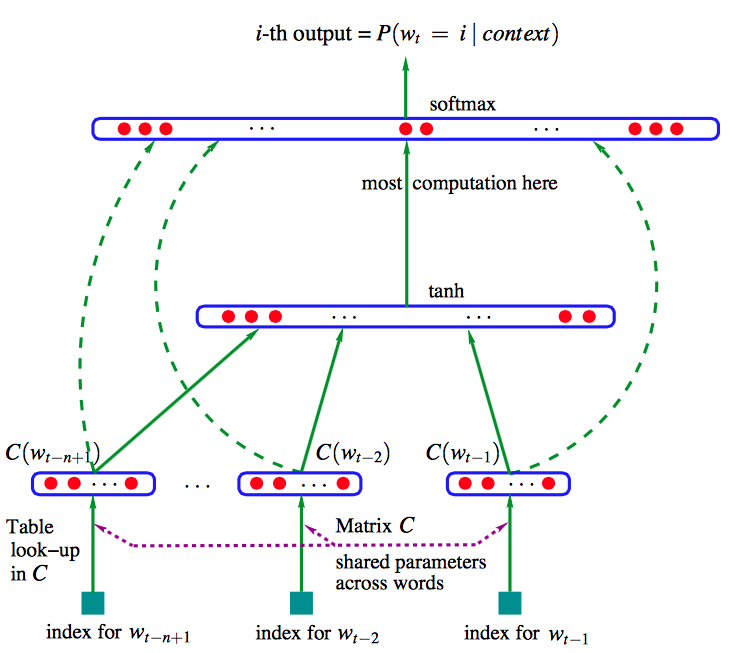
\includegraphics[width=\linewidth]{bengio_03.png}
	\caption {The first deep neural network architecture model for NLP presented by Bengio et al.}
	\label{fig:bengio_03}
\end{marginfigure}

\begin{equation}
	\hat{y} = softmax (W^{(2)} tanh(W^{(1)}x+b^{(1)})+W^{(3)}x+b^{(3)})
	\label{eqn:bengio_eqn}
\end{equation}
Note that the weight matrix $W^{(1)}$ is applied to the word vectors (solid green arrows in Figure ~\ref{fig:bengio_03}), $W^{(2)}$ is applied to the hidden layer (also solid green arrow) and $W^{(3)}$ is applied to the word vectors (dashed green arrows).

In all conventional language models, the memory requirements of the system grows exponentially with the window size $n$ making it nearly impossible to model large word windows without running out of memory.

\section{Recurrent Neural Networks (RNN)}
Unlike the conventional translation models, where only a finite window of previous words would be considered for conditioning the language model, Recurrent Neural Networks (RNN) are capable of conditioning the model on \textit{all} previous words in the corpus. 

Figure~\ref{fig:rnn} introduces the RNN architecture where rectangular box is a hidden layer at a time-step, $t$. Each such layer holds a number of neurons, each of which performing a linear matrix operation on its inputs followed by a non-linear operation (e.g. $\operatorname{tanh()}$). At each time-step, the output of the previous step along with the next word vector in the document, $x_t$, are inputs to the hidden layer to produce a prediction output $\hat{y}$ and output features $h_t$ (Equations~\ref{eqn:h_t} and \ref{eqn:y}). The inputs and outputs of each single neuron are illustrated in Figure~\ref{fig:rnn_node}.
\begin{equation}
	h_t = \sigma (W^{(hh)}h_{t-1} + W^{(hx)}x_{[t]})
	\label{eqn:h_t}
\end{equation}

\begin{equation}
	\hat{y}_t = softmax(W^{(S)}h_t)
	\label{eqn:y}
\end{equation}

\begin{marginfigure}
	\centering
	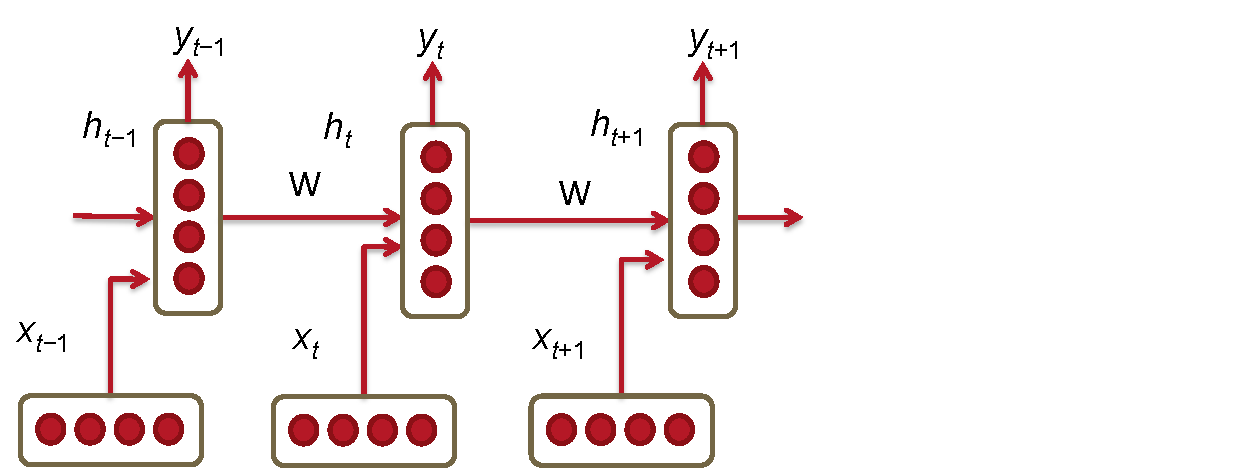
\includegraphics[width=\linewidth]{rnn.pdf}
	\caption {A Recurrent Neural Network (RNN). Three time-steps are shown.}
	\label{fig:rnn}
\end{marginfigure}

Below are the details associated with each parameter in the network:
\begin{itemize}
	\item $x_1, ..., x_{t-1}, x_t, x_{t+1}, ... x_{T}$: the word vectors corresponding to a corpus with T words.
	\item $h_t = \sigma(W^{(hh)} h_{t-1} + W^{(hx)} x_{t})$: the relationship to compute the hidden layer output features at each time-step $t$
	\begin{itemize}
		\item $x_{t} \in \mathbb{R}^{d}$: input word vector at time $t$. 
		\item $W^{hx} \in \mathbb{R}^{D_h \times d}$: weights matrix used to condition the input word vector, $x_t$
		\item $W^{hh} \in \mathbb{R}^{D_h \times D_h}$: weights matrix used to condition the output of the previous time-step, $h_{t-1}$
		\item $h_{t-1}  \in \mathbb{R}^{D_h}$: output of the non-linear function at the previous time-step, $t-1$. $h_0 \in \mathbb{R}^{D_h}$ is an initialization vector for the hidden layer at time-step $t = 0$.
		\item $\sigma ()$: the non-linearity function (sigmoid here)
	\end{itemize}
	\item $\hat{y}_t = softmax (W^{(S)}h_t)$: the output probability distribution over the vocabulary at each time-step $t$. Essentially, $\hat{y}_t$ is the next predicted word given the document context score so far (i.e. $h_{t-1}$) and the last observed word vector $x^{(t)}$. Here, $W^{(S)} \in \mathbb{R}^{|V| \times D_h}$ and $\hat{y} \in \mathbb{R}^{|V|}$ where $|V|$ is the vocabulary.
\end{itemize}

The loss function used in RNNs is often the cross entropy error introduced in earlier notes. Equation~\ref{eqn:rnn_loss} shows this function as the sum over the entire vocabulary at time-step $t$.
\begin{equation}
	J^{(t)}(\theta) = - \sum_{j=1}^{|V|} y_{t,j} \times log (\hat{y}_{t,j})
	\label {eqn:rnn_loss}
\end{equation}

The cross entropy error over a corpus of size $T$ is:
\begin{equation}
	J = \dfrac{1}{T} \sum_{t=1}^{T} J^{(t)}(\theta) = - \dfrac{1}{T} \sum_{t=1}^{T} \sum_{j=1}^{|V|} y_{t,j} \times log (\hat{y}_{t,j})
	\label {eqn:rnn_loss_T}
\end{equation}

\begin{marginfigure}
	\centering
	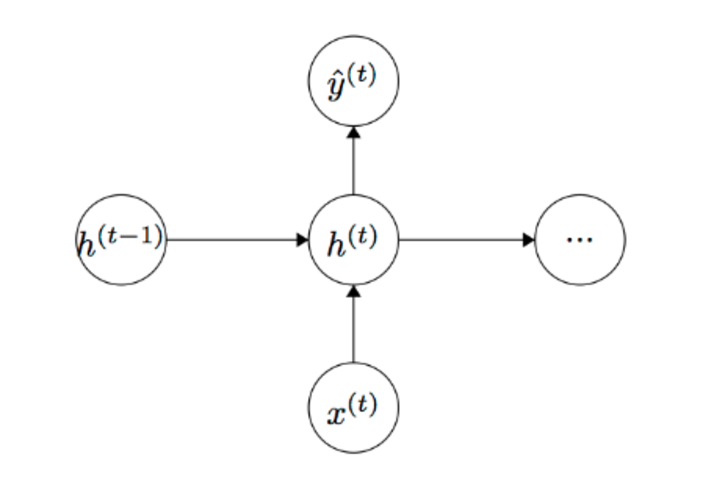
\includegraphics[width=\linewidth]{rnn_node.pdf}
	\caption {The inputs and outputs to a neuron of a RNN}
	\label{fig:rnn_node}
\end{marginfigure}


Equation~\ref{eqn:perplexity} is called the \textit{perplexity} relationship; it is basically 2 to the power of the negative log probability of the cross entropy error function shown in Equation~\ref{eqn:rnn_loss_T}. Perplexity is a measure of confusion where lower values imply more confidence in predicting the next word in the sequence (compared to the ground truth outcome).

\begin{equation}
	Perplexity = 2^{J}
	\label{eqn:perplexity}
\end{equation}

The amount of memory required to run a layer of RNN is proportional to the number of words in the corpus. For instance, a sentence with k words would have k word vectors to be stored in memory. Also, the RNN must maintain two pairs of  $W, b$ matrices. While the size of W could be very large, it does not scale with the size of the corpus (unlike the traditional language models). For a RNN with 1000 recurrent layers, the matrix would be $1000 \times 1000$ regardless of the corpus size.

Figure~\ref{fig:rnn_loop} is an alternative representation of RNNs used in some publications. It represents the RNN hidden layer as a loop.
\begin{marginfigure}
	\centering
	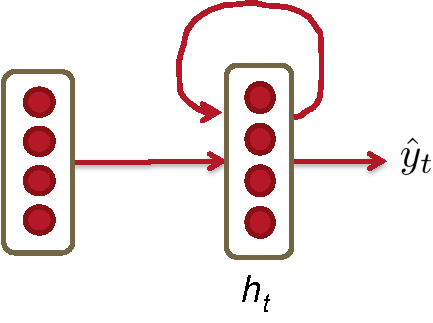
\includegraphics[width=\linewidth]{rnn_loop.pdf}
	\caption {The illustration of a RNN as a loop over time-steps}
	\label{fig:rnn_loop}
\end{marginfigure}

%\subsection{RNN Training}
%Training RNN is specifically difficult because ?

\subsection{Vanishing Gradient \& Gradient Explosion Problems}
Recurrent neural networks propagate weight matrices from one time-step to the next. Recall the goal of a RNN implementation is to enable propagating context information through faraway time-steps. For example, consider the following two sentences:

\null
\centering
\uline{Sentence 1}

"Jane walked into the room. John walked in too. Jane said hi to \_\_\_"

\null
\uline{Sentence 2}

"Jane walked into the room. John walked in too. It was late in the day, and everyone was walking home after a long day at work. Jane said hi to \_\_\_"

\null
\justify
In both sentences, given their context, one can tell the answer to both blank spots is most likely "John". It is important that the RNN predicts the next word as "John", the second person who has appeared several time-steps back in both contexts. Ideally, this should be possible given what we know about RNNs so far. In practice, however, it turns out RNNs are more likely to correctly predict the blank spot in Sentence 1 than in Sentence 2. This is because during the back-propagation phase, the contribution of gradient values gradually vanishes as they propagate to earlier time-steps. Thus, for long sentences, the probability that "John" would be recognized as the next word reduces with the size of the context. Below, we discuss the mathematical reasoning behind the vanishing gradient problem.

Consider Equations~\ref{eqn:h_t} and \ref{eqn:y} at a time-step $t$; to compute the RNN error, $dE/dW$, we sum the error at each time-step. That is, $dE_t/dW$ for every time-step, $t$, is computed and accumulated.
\begin{equation}
	\dfrac{\partial E}{\partial W} = \sum_{t=1}^{T}\dfrac{\partial E_t}{\partial W}
	\label{eqn:bp_rnn_error}
\end{equation}

The error for each time-step is computed through applying the chain rule differentiation to Equations~\ref{eqn:y} and \ref{eqn:h_t}; Equation~\ref{eqn:bp_rnn_chain} shows the corresponding differentiation. Notice $dh_t/dh_k$ refers to the partial derivative of $h_t$ with respect to \textit{all} previous $k$ time-steps. 
\begin{equation}
	\dfrac{\partial E_t}{\partial W} = \sum_{k=1}^{t} \dfrac{\partial E_t}{\partial y_t} \dfrac{\partial y_t}{\partial h_t} \dfrac{\partial h_t}{\partial h_k} \dfrac{\partial h_k}{\partial W}
	\label{eqn:bp_rnn_chain}
\end{equation}

Equation~\ref{eqn:bp_rnn_k} shows the relationship to compute each $dh_t/dh_k$; this is simply a chain rule differentiation over all hidden layers within the $[k, t]$ time interval. 
\begin{equation}
	\dfrac{\partial h_t}{\partial h_k} = \prod_{j=k+1}^{t}\dfrac{\partial h_j}{\partial h_{j-1}} = \prod_{j=k+1}^{t}W^T \times diag [f'(j_{j-1})]
	\label{eqn:bp_rnn_k}
\end{equation}

Because $h \in \mathbb{R}^{D_n}$, each $\partial h_j/\partial h_{j-1}$ is the Jacobian matrix for $h$:
\begin{equation}
	\dfrac{\partial h_j}{\partial h_{j-1}} = {[\dfrac{\partial h_{j}}{\partial h_{j-1,1}} ...  \dfrac{\partial h_{j}}{\partial h_{j-1,D_n}}]} = 
	\begin{bmatrix}
	\dfrac{\partial h_{j,1}}{\partial h_{j-1,1}} & . & . & . & \dfrac{\partial h_{j,1}}{\partial h_{j-1,D_n}} \\
	. & . & & & . \\
	. & & . & & . \\
	. & & & . & . \\
	\dfrac{\partial h_{j,D_n}}{\partial h_{j-1,1}} & . & . & . & \dfrac{\partial h_{j,D_n}}{\partial h_{j-1,D_n}} \\
	\end{bmatrix}
	\label{eqn:bp_rnn_jaocb}
\end{equation}

Putting Equations~\ref{eqn:bp_rnn_error}, \ref{eqn:bp_rnn_chain}, \ref{eqn:bp_rnn_k} together, we have the following relationship.
\begin{equation}
	\dfrac{\partial E}{\partial W} = \sum_{t=1}^{T}\sum_{k=1}^{t} \dfrac{\partial E_t}{\partial y_t} \dfrac{\partial y_t}{\partial h_t} (\prod_{j=k+1}^{t}\dfrac{\partial h_j}{\partial h_{j-1}}) \dfrac{\partial h_k}{\partial W}
\end{equation}

Equation~\ref{eqn:bp_rnn_k_norm} shows the norm of the Jacobian matrix relationship in Equation~\ref{eqn:bp_rnn_jaocb}. Here, $\beta_W$ and $\beta_h$ represent the upper bound values for the two matrix norms. The norm of the partial gradient at each time-step, $t$, is therefore, calculated through the relationship shown in Equation~\ref{eqn:bp_rnn_k_norm}.

\begin {equation}
	\parallel \dfrac{\partial h_j}{\partial h_{j-1}} \parallel \leq \parallel W^T\parallel  \parallel diag [f'(h_{j-1})]\parallel \leq \beta_W \beta_h
	\label{eqn:bp_rnn_k_norm}
\end {equation}

The norm of both matrices is calculated through taking their L2-norm. The norm of $f'(h_{j-1})$ can only be as large as 1 given the sigmoid non-linearity function.

\begin {equation}
	\parallel \dfrac{\partial h_t}{\partial h_k} \parallel = \parallel \prod_{j=k+1}^{t} \dfrac{\partial h_j}{\partial h_{j-1}}\parallel \leq (\beta_W \beta_h)^{t-k}
	\label{eqn:bp_rnn_k_norm_total}
\end {equation}

The exponential term $(\beta_W \beta_h)^{t-k}$ can easily become a very small or large number when $\beta_W \beta_h$ is much smaller or larger than 1 and $t-k$ is sufficiently large. Recall a large $t-k$ evaluates the cross entropy error due to faraway words. The contribution of faraway words to predicting the next word at time-step $t$ diminishes when the gradient vanishes early on.

During experimentation, once the gradient value grows extremely large, it causes an overflow (i.e. NaN) which is easily detectable at runtime; this issue is called the \textit{Gradient Explosion Problem}. When the gradient value goes to zero, however, it can go undetected while drastically reducing the learning quality of the model for far-away words in the corpus; this issue is called the \textit{Vanishing Gradient Problem}.

To gain practical intuition about the vanishing gradient problem, you may visit the following \uline{\href{http://cs224d.stanford.edu/notebooks/vanishing_grad_example.html}{example website}}.

\subsection{Solution to the Exploding \& Vanishing Gradients}
Now that we gained intuition about the nature of the vanishing gradients problem and how it manifests itself in deep neural networks, let us focus on a simple and practical heuristic to solve these problems. 

To solve the problem of exploding gradients, Thomas Mikolov first introduced a simple heuristic solution that \textit{clips} gradients to a small number whenever they explode. That is, whenever they reach a certain threshold, they are set back to a small number as shown in Algorithm~\ref{alg:clip}.

\begin{algorithm}
\begin{algorithmic}
\State $\hat{g} \gets \dfrac{\partial E}{\partial W}$
\If {$\parallel \hat{g} \parallel \geq threshold$}
    \State $\hat{g} \gets \dfrac{threshold}{\parallel \hat{g} \parallel} \hat{g}$
\EndIf
\end{algorithmic}
\caption{Psudo-code for norm clipping in the gradients whenever they explode}
\label{alg:clip}
\end{algorithm}

Figure~\ref{fig:clipping} visualizes the effect of gradient clipping. It shows the decision surface of a small recurrent neural network with respect to its $W$ matrix and its bias terms, $b$. The model consists of a single unit of recurrent neural network running through a small number of time-steps; the solid arrows illustrate the training progress on each gradient descent step. When the gradient descent model hits the high error wall in the objective function, the gradient is pushed off to a far-away location on the decision surface. The clipping model produces the dashed line where it instead pulls back the error gradient to somewhere close to the original gradient landscape.

\begin{marginfigure}
	\centering
	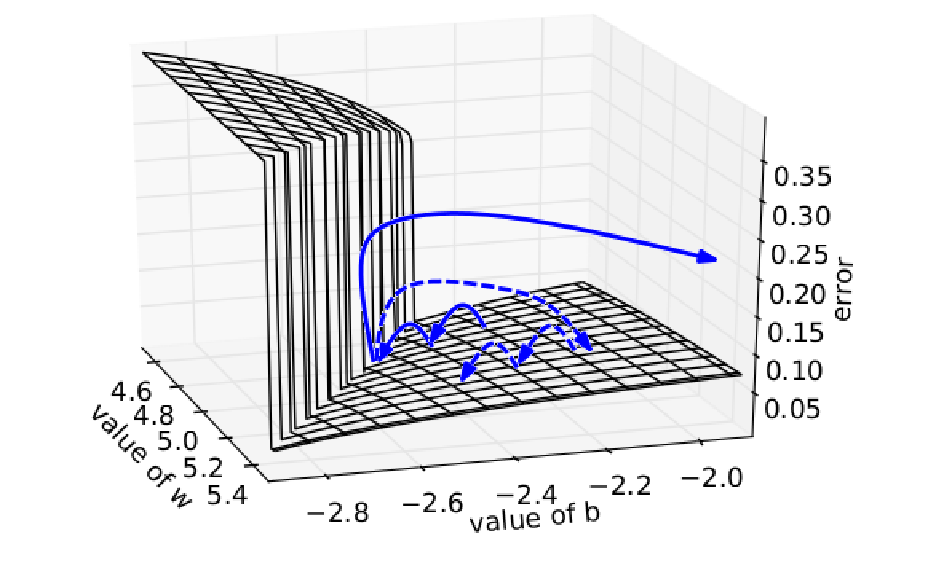
\includegraphics[width=\linewidth]{cliping.pdf}
	\caption {Gradient explosion clipping visualization}
	\label{fig:clipping}
\end{marginfigure}

To solve the problem of vanishing gradients, we introduce two techniques. The first technique is that instead of initializing $W^{(hh)}$ randomly, start off from an identify matrix initialization. 
%TODO the initialization idea requires more writing

The second technique is to use the Rectified Linear Units (ReLU) instead of the sigmoid function. The derivative for the ReLU is either 0 or 1. This way, gradients would flow through the neurons whose derivative is 1 without getting attenuated while propagating back through time-steps.


\subsection{Deep Bidirectional RNNs}
So far, we have focused on RNNs that look into the past words to predict the next word in the sequence. It is possible to make predictions based on future words by having the RNN model read through the corpus backwards. Irsoy et al. shows a bi-directional deep neural network; at each time-step, $t$, this network maintains two hidden layers, one for the left-to-right propagation and another for the right-to-left propagation. To maintain two hidden layers at any time, this network consumes twice as much memory space for its weight and bias parameters. The final classification result, $\hat{y_t}$, is generated through combining the score results produced by both RNN hidden layers. Figure~\ref{fig:birnn} shows the bi-directional network architecture, and Equations~\ref{eqn:rnn_right} and \ref{eqn:rnn_left} show the mathematical formulation behind setting up the bi-directional RNN hidden layer. The only difference between these two relationships is in the direction of recursing through the corpus. Equation~\ref{eqn:birnn_classifier} shows the classification relationship used for predicting the next word via summarizing past and future word representations.

\begin{marginfigure}
	\centering
	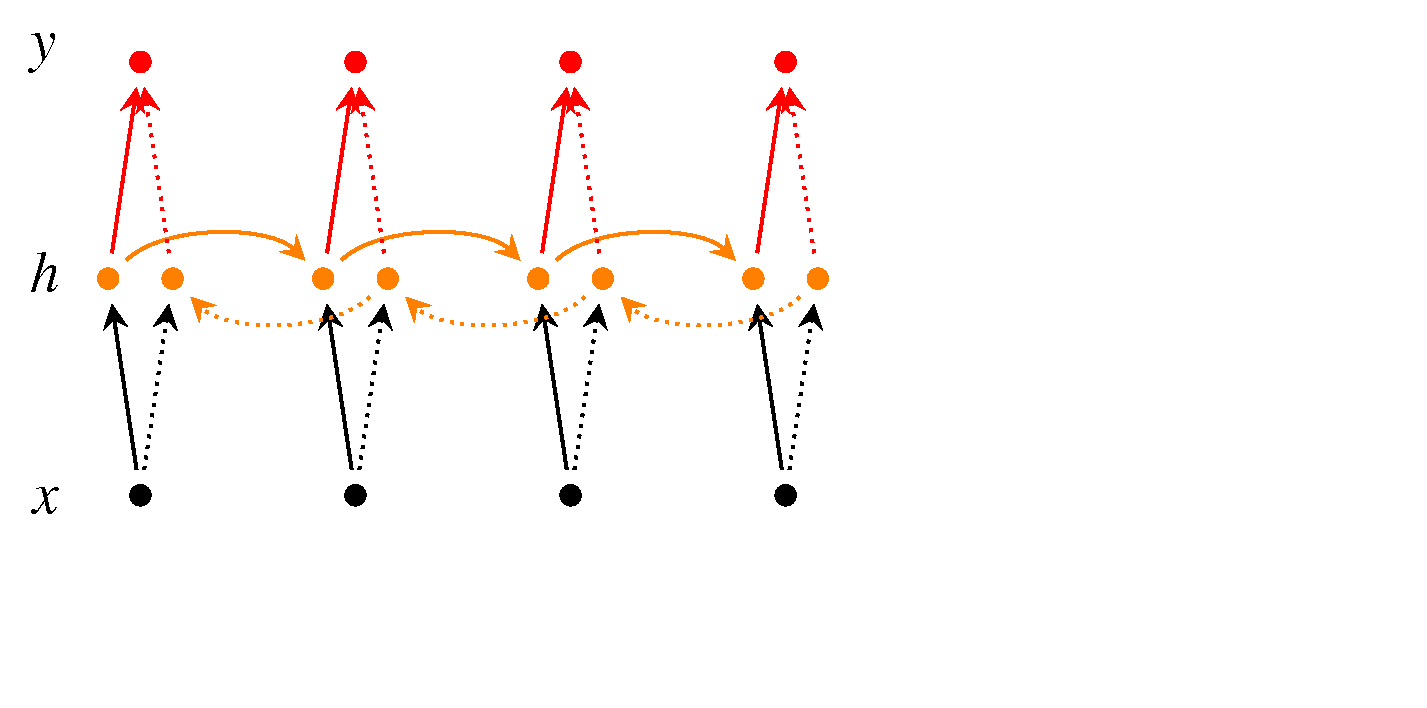
\includegraphics[width=\linewidth]{birnn.pdf}
	\caption {A bi-directional RNN model}
	\label{fig:birnn}
\end{marginfigure}

\begin{equation}
	\overrightarrow{h}_t = f(\overrightarrow{W} x_t + \overrightarrow{V} \overrightarrow{h}_{t-1} + \overrightarrow{b})
	\label{eqn:rnn_right}
\end{equation}
\begin{equation}
	\overleftarrow{h}_t = f(\overleftarrow{W} x_t + \overleftarrow{V} \overleftarrow{h}_{t+1} + \overleftarrow{b})
	\label{eqn:rnn_left}
\end{equation}
\begin{equation}
	\hat{y}_t = g(U h_t + c) = g(U [\overrightarrow{h}_t; \overleftarrow{h}_t] + c)
	\label{eqn:birnn_classifier}
\end{equation}

Figure~\ref{fig:deepbirnn} shows a multi-layer bi-directional RNN where each lower layer feeds the next layer. As shown in this figure, in this network architecture, at time-step $t$ each intermediate neuron receives one set of parameters from the previous time-step (in the same RNN layer), and two sets of parameters from the previous RNN hidden layer; one input comes from the left-to-right RNN and the other from the right-to-left RNN.  

To construct a Deep RNN with $L$ layers, the above relationships are modified to the relationships in Equations~\ref{eqn:d_rnn_right} and \ref{eqn:d_rnn_left} where the input to each intermediate neuron at level $i$ is the output of the RNN at layer $i-1$ at the same time-step, $t$. The output, $\hat{y}$, at each time-step is the result of propagating input parameters through all hidden layers (Equation~\ref{eqn:d_birnn_classifier}).

\begin{marginfigure}
	\centering
	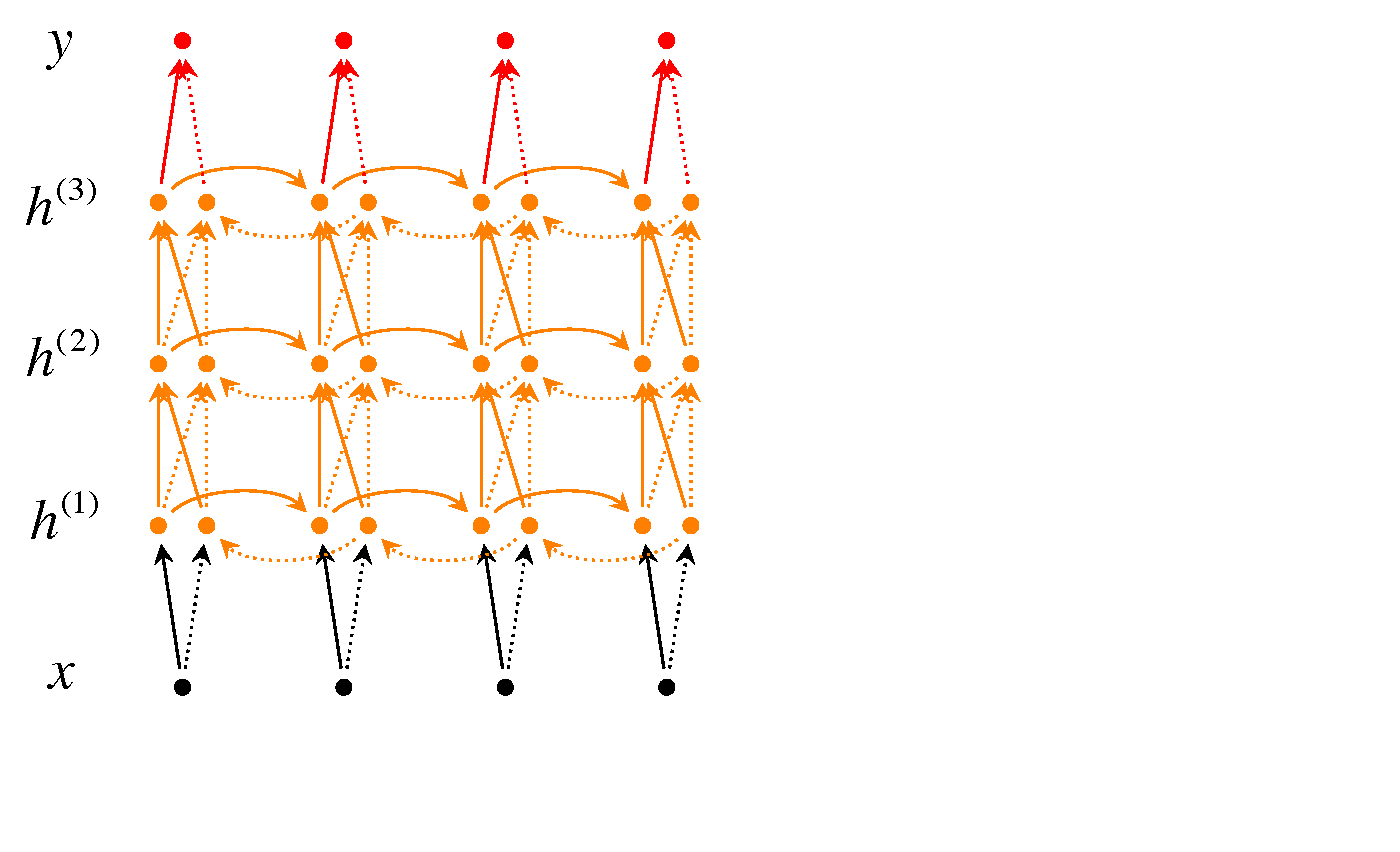
\includegraphics[width=\linewidth]{deepbirnn.pdf}
	\caption {A deep bi-directional RNN with three RNN layers.}
	\label{fig:deepbirnn}
\end{marginfigure}

\begin{equation}
	\overrightarrow{h}_t^{(i)} = f(\overrightarrow{W}^{(i)} h_t^{(i-1)} + \overrightarrow{V}^{(i)} \overrightarrow{h}_{t-1}^{(i)} + \overrightarrow{b}^{(i)})
	\label{eqn:d_rnn_right}
\end{equation}
\begin{equation}
	\overleftarrow{h}_t^{(i)} = f(\overleftarrow{W}^{(i)} h_t^{(i-1)} + \overleftarrow{V}^{(i)} \overleftarrow{h}_{t+1}^{(i)} + \overleftarrow{b}^{(i)})
	\label{eqn:d_rnn_left}
\end{equation}
\begin{equation}
	\hat{y}_t = g(U h_t + c) = g(U [\overrightarrow{h}_t^{(L)}; \overleftarrow{h}_t^{(L)}] + c)
	\label{eqn:d_birnn_classifier}
\end{equation}

\subsection{Application: RNN Translation Model}
Traditional translation models are quite complex; they consist of numerous machine learning algorithms applied to different stages of the language translation pipeline. In this section, we discuss the potential for adopting RNNs as a replacement to traditional translation modules. Consider the RNN example model shown in Figure~\ref{fig:rnn_translate}; here, the German phrase \textit{Echt dicke Kiste} is translated to \textit{Awesome sauce}. The first three hidden layer time-steps \textit{encode} the German language words into some language word features ($h_3$). The last two time-steps \textit{decode} $h_3$ into English word outputs. Equation~\ref{eqn:encoder} shows the relationship for the Encoder stage and Equations~\ref{eqn:decoder_h} and \ref{eqn:decoder_y} show the equation for the Decoder stage.

\begin{marginfigure}
	\centering
	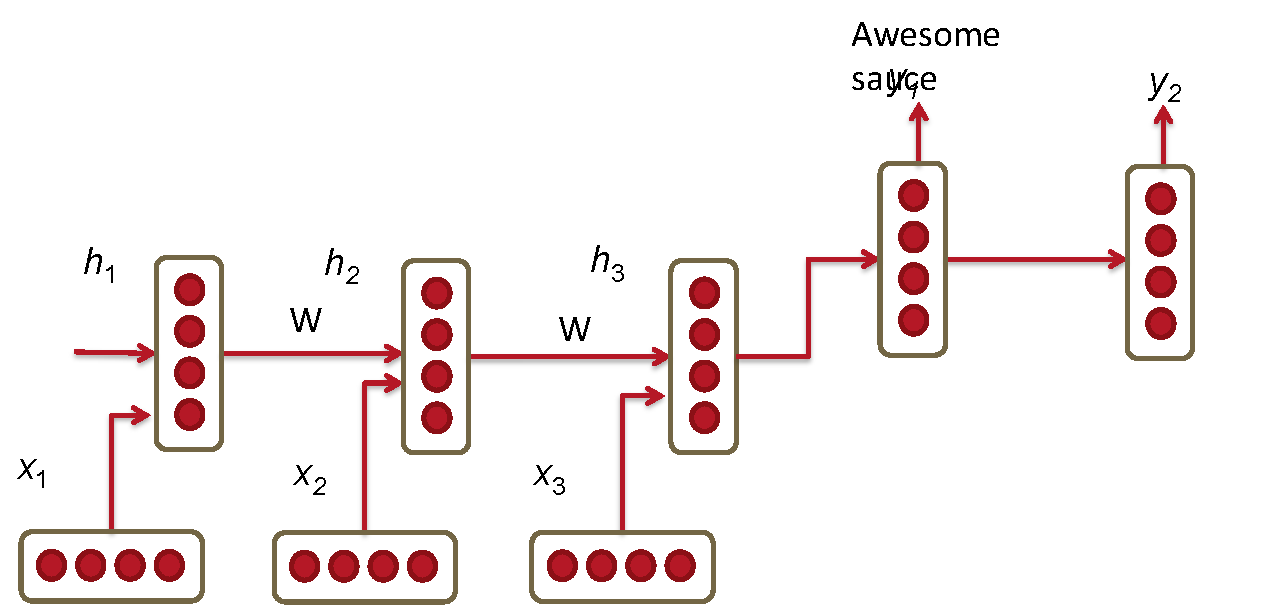
\includegraphics[width=\linewidth]{rnn_translate.pdf}
	\caption {A RNN-based translation model. The first three RNN hidden layers belong to the source language model encoder, and the last two belong to the destination language model decoder.}
	\label{fig:rnn_translate}
\end{marginfigure}

\begin{equation}
	h_t = \phi (h_{t-1}, x_t) = f (W^{(hh)} h_{t-1} + W^{(hx)} x_t)
	\label{eqn:encoder}
\end{equation}

\begin{equation}
	h_t = \phi (h_{t-1}) = f (W^{(hh)} h_{t-1})
	\label{eqn:decoder_h}
\end{equation}
\begin{equation}
	y_t = softmax (W^{(S)}h_t)
	\label{eqn:decoder_y}
\end{equation}

One may naively assume this RNN model along with the cross-entropy function shown in Equation~\ref{eqn:decoder_ce} can produce high-accuracy translation results. In practice, however, several extensions are to be added to the model to improve its translation accuracy performance.

\begin{equation}
	\max_{\theta} \dfrac {1}{N} \sum_{n=1}^{N} \log p_{\theta} (y^{(n)}|x^{(n)})
	\label{eqn:decoder_ce}
\end{equation}

\paragraph{Extension I:} train different RNN weights for encoding and decoding. This decouples the two units and allows for more accuracy prediction of each of the two RNN modules. This means the $\phi()$ functions in Equations~\ref{eqn:encoder} and \ref{eqn:decoder_h} would have different $W^{(hh)}$ matrices.

\paragraph{Extension II:} compute every hidden state in the decoder using three different inputs:

\begin{itemize}
	\item The previous hidden state (standard)
	\item  Last hidden layer of the encoder ($c = h_T$ in Figure~\ref{fig:en_decoder})
	\item Previous predicted output word, $\hat{y}_{t-1}$
\end{itemize}

\begin{marginfigure}
	\centering
	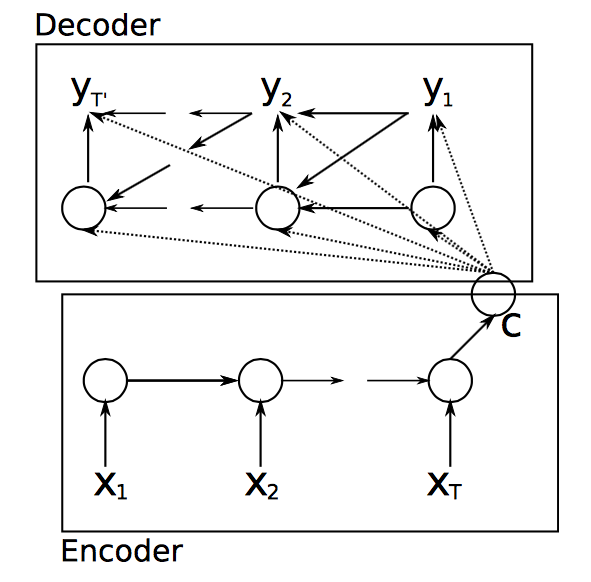
\includegraphics[width=\linewidth]{en_decoder.png}
	\caption {Language model with three inputs to each decoder neuron: ($h_{t-1}, c, y_{t-1}$)}
	\label{fig:en_decoder}
\end{marginfigure}

Combining the above three inputs transforms the $\phi$ function in the decoder function of Equation~\ref{eqn:decoder_h} to the one in Equation~\ref{eqn:decoder_hs}. Figure~\ref{fig:en_decoder} illustrates this model.

\begin{equation}
	h_{t} = \phi (h_{t-1}, c, y_{t-1})
	\label{eqn:decoder_hs}
\end{equation}

\paragraph{Extension III:} train deep recurrent neural networks using multiple RNN layers as discussed earlier in this chapter. Deeper layers often improve prediction accuracy due to their higher learning capacity. Of course, this implies a large training corpus must be used to train the model.

\paragraph{Extension IV:} train bi-directional encoders to improve accuracy similar to what was discussed earlier in this chapter.

\paragraph{Extension V:} given a word sequence  \textit{A B C} in German whose translation is \textit{X Y} in English, instead of training the RNN using \textit{A B C} $\to$ \textit{X Y}, train it using \textit{C B A} $\to$ \textit{X Y}. The intutition behind this technique is that \textit{A} is more likely to be translated to \textit{X}. Thus, given the vanishing gradient problem discussed earlier, reversing the order of the input words can help reduce the error rate in generating the output phrase.

\section{Gated Recurrent Units}\label{sec:grus}
Beyond the extensions discussed so far, RNNs have been found to perform better with the use of more complex units for activation. So far, we have discussed methods that transition from hidden state $h_{t-1}$ to $h_{t}$ using an affine transformation and a point-wise nonlinearity. Here, we discuss the use of a gated activation function thereby modifying the RNN architecture. What motivates this? Well, although RNNs can theoretically capture long-term dependencies, they are very hard to actually train to do this. Gated recurrent units are designed in a manner to have more persistent memory thereby making it easier for RNNs to capture long-term dependencies. Let us see mathematically how a GRU uses $h_{t-1}$ and $x_{t}$ to generate the next hidden state $h_{t}$. We will then dive into the intuition of this architecture.
\begin{align*}
z_{t} &= \sigma(W^{(z)}x_{t} + U^{(z)}h_{t-1})&~\text{(Update gate)}\\
r_{t} &= \sigma(W^{(r)}x_{t} + U^{(r)}h_{t-1})&~\text{(Reset gate)}\\
\tilde{h}_{t} &= \operatorname{tanh}(r_{t}\circ  Uh_{t-1} + Wx_{t} )&~\text{(New memory)}\\
h_{t} &= (1 - z_{t}) \circ \tilde{h}_{t} + z_{t} \circ h_{t-1}&~\text{(Hidden state)}
\end{align*}
The above equations can be thought of a GRU's four fundamental operational stages and they have intuitive interpretations that make this model much more intellectually satisfying (see Figure~\ref{fig:GRU}):
\begin{enumerate}
\item \textbf{New memory generation:} A new memory $\tilde{h}_{t}$ is the consolidation of a new input word $x_{t}$ with the past hidden state $h_{t-1}$. Anthropomorphically, this stage is the one who knows the recipe of combining a newly observed word with the past hidden state $h_{t-1}$ to summarize this new word in light of the contextual past as the vector $\tilde{h}_{t}$.
\item \textbf{Reset Gate:} The reset signal $r_{t}$ is responsible for determining how important $h_{t-1}$ is to the summarization $\tilde{h}_{t}$. The reset gate has the ability to completely diminish past hidden state if it finds that $h_{t-1}$ is irrelevant to the computation of the new memory.
\item \textbf{Update Gate:} The update signal $z_{t}$ is responsible for determining how much of $h_{t-1}$ should be carried forward to the next state. For instance, if $z_{t} \approx 1$, then $h_{t-1}$ is almost entirely copied out to $h_{t}$. Conversely, if $z_{t} \approx 0$, then mostly the new memory $\tilde{h}_{t}$ is forwarded to the next hidden state.
\item \textbf{Hidden state:} The hidden state $h_{t}$ is finally generated using the past hidden input $h_{t-1}$ and the new memory generated $\tilde{h}_{t}$ with the advice of the update gate.
\end{enumerate}

\begin{figure*}%
  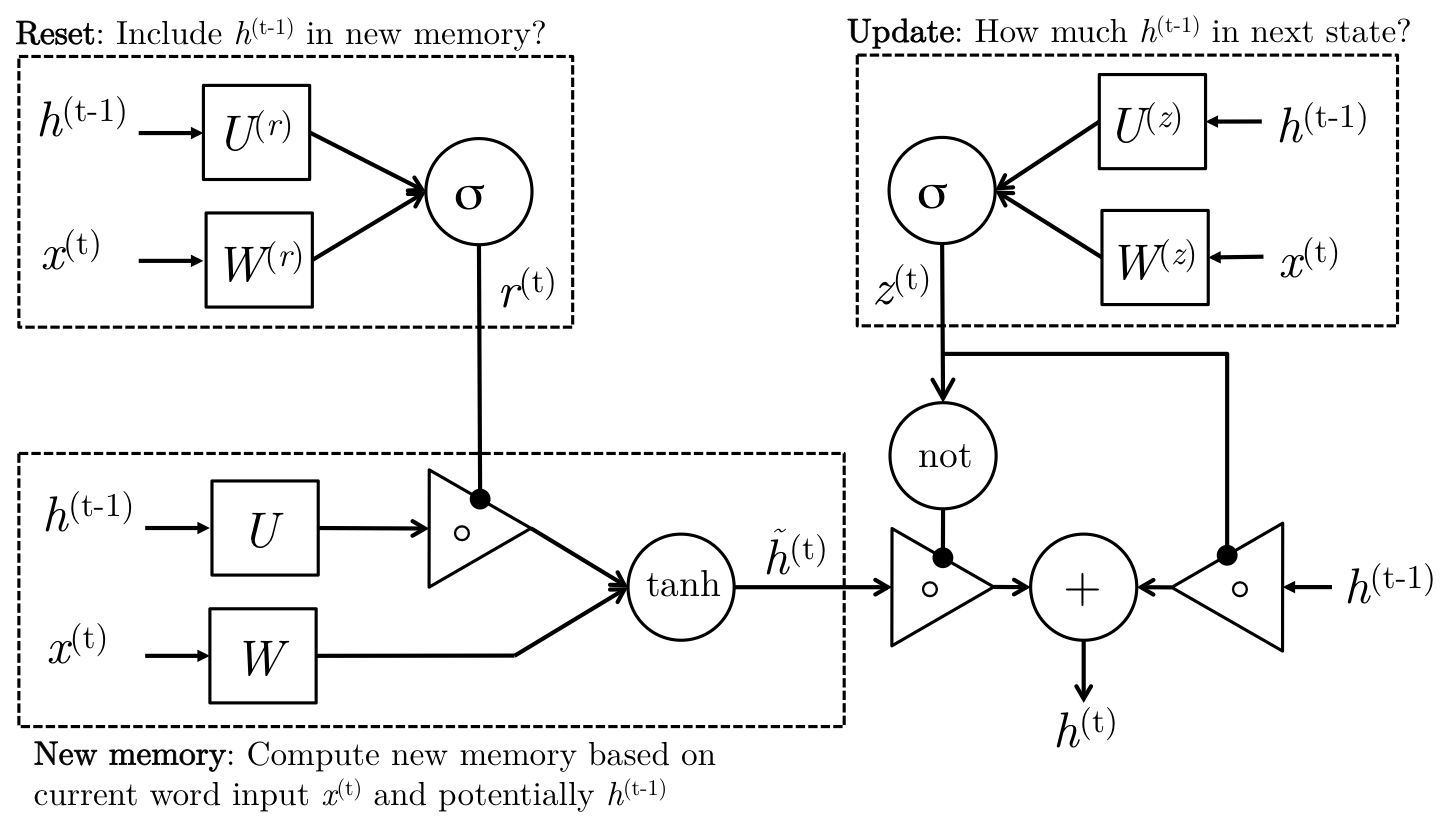
\includegraphics[width = 15cm]{GRU}
  \caption{The detailed internals of a GRU}
  \label{fig:GRU}
\end{figure*}

It is important to note that to train a GRU, we need to learn all the different parameters: $W, U, W^{(r)}, U^{(r)}, W^{(z)}, U^{(z)}$. These follow the same backpropagation procedure we have seen in the past.

\section{Long-Short-Term-Memories}\label{sec:lstm}

Long-Short-Term-Memories are another type of complex activation unit that differ a little from GRUs. The motivation for using these is similar to those for GRUs however the architecture of such units does differ. Let us first take a look at the mathematical formulation of LSTM units before diving into the intuition behind this design:
\begin{align*}
i_{t} &= \sigma(W^{(i)}x_{t} + U^{(i)}h_{t-1})&~\text{(Input gate)}\\
f_{t} &= \sigma(W^{(f)}x_{t} + U^{(f)}h_{t-1})&~\text{(Forget gate)}\\
o_{t} &= \sigma(W^{(o)}x_{t} + U^{(o)}h_{t-1})&~\text{(Output/Exposure gate)}\\
\tilde{c}_{t} &= \operatorname{tanh}(W^{(c)}x_{t} + U^{(c)}h_{t-1})&~\text{(New memory cell)}\\
c_{t} &= f_{t} \circ c_{t-1} + i_{t} \circ \tilde{c}_{t}&~\text{(Final memory cell)}\\
h_{t} &= o_{t} \circ \operatorname{tanh}(c_{t}) 
\end{align*}

\begin{figure*}%
  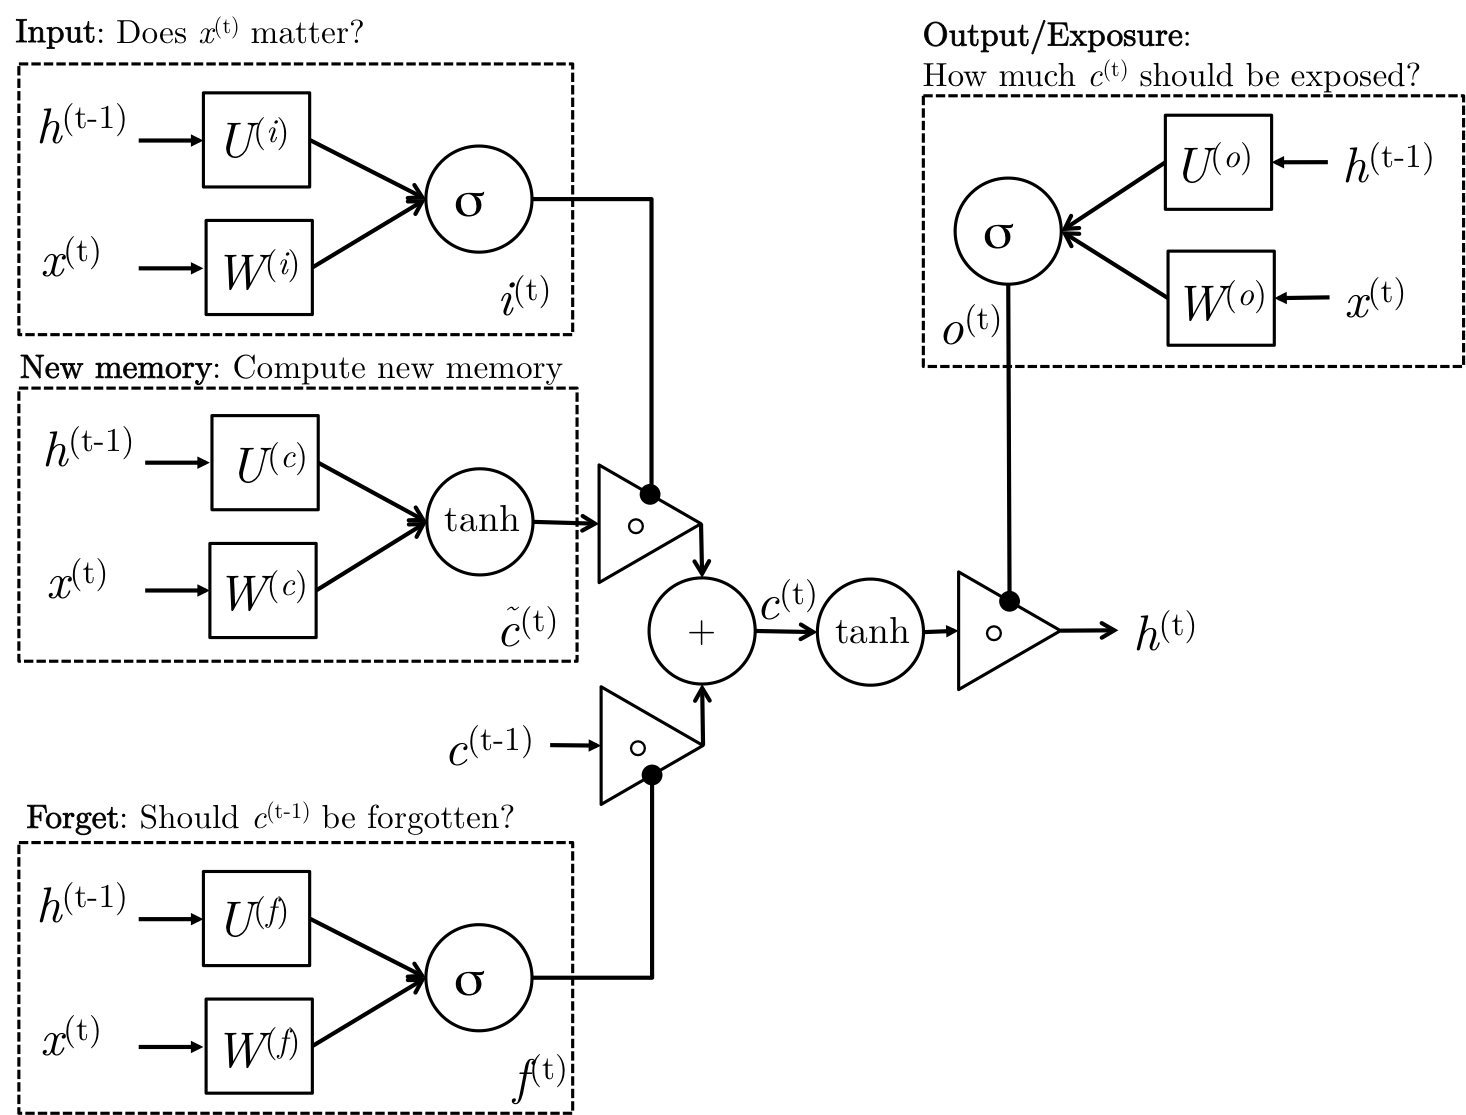
\includegraphics[width = 15cm]{LSTM}
  \caption{The detailed internals of a LSTM}
  \label{fig:LSTM}
\end{figure*}

We can gain intuition of the structure of an LSTM by thinking of its architecture as the following stages:
\begin{enumerate}
\item \textbf{New memory generation:} This stage is analogous to the new memory generation stage we saw in GRUs. We essentially use the input word $x_{t}$ and the past hidden state $h_{t-1}$ to generate a new memory $\tilde{c}_{t}$ which includes aspects of the new word $x^{(t)}$.
\item \textbf{Input Gate:} We see that the new memory generation stage doesn't check if the new word is even important before generating the new memory -- this is exactly the input gate's function. The input gate uses the input word and the past hidden state to determine whether or not the input is worth preserving and thus is used to gate the new memory. It thus produces $i_{t}$ as an indicator of this information.
\item \textbf{Forget Gate:} This gate is similar to the input gate except that it does not make a determination of usefulness of the input word -- instead it makes an assessment on whether the past memory cell is useful for the computation of the current memory cell. Thus, the forget gate looks at the input word and the past hidden state and produces $f_{t}$.
\item \textbf{Final memory generation:} This stage first takes the advice of the forget gate $f_{t}$ and accordingly forgets the past memory $c_{t-1}$. Similarly, it takes the advice of the input gate $i_{t}$ and accordingly gates the new memory $\tilde{c}_{t}$. It then sums these two results to produce the final memory $c_{t}$.
\item \textbf{Output/Exposure Gate:} This is a gate that does not explicitly exist in GRUs. It's purpose is to separate the final memory from the hidden state. The final memory $c_{t}$ contains a lot of information that is not necessarily required to be saved in the hidden state. Hidden states are used in every single gate of an LSTM and thus, this gate makes the assessment regarding what parts of the memory $c_{t}$ needs to be exposed/present in the hidden state $h_{t}$. The signal it produces to indicate this is $o_{t}$ and this is used to gate the point-wise tanh of the memory.
\end{enumerate}

\end{document}